
% \usepackage{amsthm}
% \theoremstyle{plain}
\newtheorem{lemma}{Lemma}
\newtheorem{sublemma}{Lemma}[lemma]
\newtheorem{theorem}{Theorem}[section]

\section{Background}
% \blindtext
This section is designed to give an the numerical tools for construction optimizations for MSSC. It will first cover on of the more traditional methods before giving an overview on how DC programming may be adapted as well. 
% \subsection{Literature Review}


\subsection{Mean Sum of Squares}
Square error algorithms, such as Mean Sum of Squares (MSSC), are some of the most frequently used classical methods for clustering data of distinct sets. These usually take the form of minimizing the distance between a set of n points/entities within a $c$ clusters to each cluster's centroid. For convenience, we will present using the notation present in \cite{an_minimum_2009}. Mathematically, this can be formulated as having $n$ entities be denoted as \(X := \{x_1, x_2, \ldots, x_n\} \in \mathbb{R}^d\). These are partitioned into \(c (2\le c\le n) \) clusters. The identification of which cluster element \(n\) is part of can be easily represented as \(U = (u_{i,k}) \in \mathbb{R}^{c\times n}\) with \(i =1,...,c\) and \(k =1,...,n.\) or as



    % Definition of the assignment variables
\[
u_{i,k} :=
\begin{cases}
1, & \text{if } x_k \in C_i,\\
0, & \text{otherwise}.
\end{cases}
\]
\noindent Further, with centriods $v_i \in \mathbb{R}^d$ and  the matrix \(V \in \mathbb{R}^{c\times d}\) where each column is $v_i$, MSSC can be formulated as 
% MSSC formulation
% \begin{equation}
\begin{equation}
\begin{cases}
\min{ f(U,V)}
:=  \sum_{k=1}^n \sum_{i=1}^c u_{i,k} \,\bigl\lVert x_k - v_i\bigr\rVert^2, \\[8pt]
\text{s.t.}\quad
u_{i,k} \in \{0,1\}, 
\quad i = 1,\dots,c,\; k = 1,\dots,n,\\[8pt]
\sum_{i=1}^c u_{i,k} = 1,\quad k = 1,\dots,n.
\end{cases}\\
\label{eq:my_equatio}
\end{equation}

\noindent These formulations can be uses with several optimization algorithms such as K-means and DCA.


\subsection{K-means}
%cover overview ith algorithm --baseline comparison 
One of the benchmark algorithms in clustering is the K-means algorithm introduced in \cite{macqueen_methods_1967}, and is time complexity of \(O(n)\) \cite{jain_data_1999}. One problem with this algorithm is that it is sensitive to its initialization and does not guarantee convergence to a global minimum. The basic implementation is shown in Algorithm \ref{alg:kmeans}. Example results shown in figure \ref{fig:kmeans}.


% \begin{figure}[!htpb]
%     \centering
%     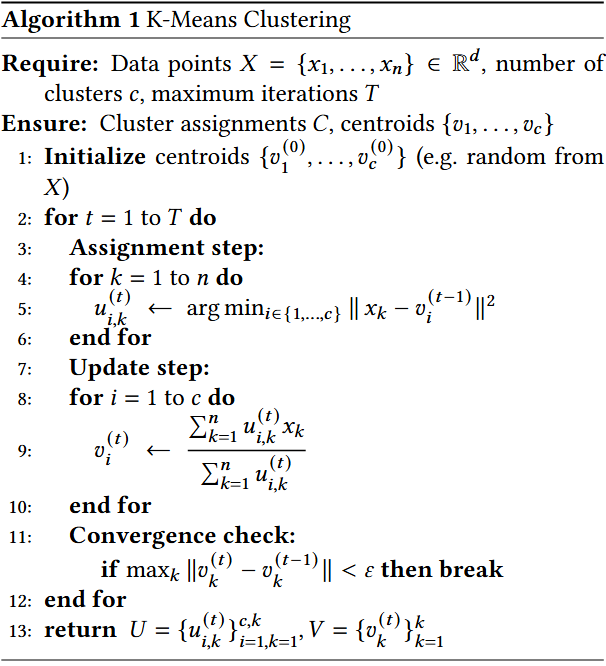
\includegraphics[width=\linewidth]{Figures/K-means_clustering.png}
%     \label{alg:kmeans}
% \end{figure}

\begin{algorithm}[ht]
\caption{K‐Means Clustering}
\label{alg:kmeans}
\begin{algorithmic}[1]
\REQUIRE Data points $X = \{x_1, \ldots, x_n\}\in\mathbb{R}^d$, number of clusters $c$, maximum iterations $T$
\ENSURE Cluster assignments $C$, centroids $\{v_1,\dots,v_c\}$
\STATE \textbf{Initialize} centroids $\{v_1^{(0)},\dots,v_c^{(0)}\}$ (e.g.\ random from $X$)
\FOR{$t = 1$ to $T$}
  \STATE \textbf{Assignment step:}
  \FOR{$k = 1$ to $n$}
    \STATE $u_{i,k}^{(t)} \;\leftarrow\; \arg\min_{i\in\{1,\dots,c\}}\|\,x_k - v_i^{(t-1)}\|^2$
  \ENDFOR
  \STATE \textbf{Update step:}
  \FOR{$i = 1$ to $c$}
    \STATE $\displaystyle v_i^{(t)} 
      \;\leftarrow\; 
      \frac{\sum_{k=1}^nu_{i,k}^{(t)}x_k}{\sum_{k=1}^nu_{i,k}^{(t)}}$
  \ENDFOR
  \STATE \textbf{Convergence check:} \\
    \hspace*{1em} \textbf{if} $\max_k \|v_k^{(t)} - v_k^{(t-1)}\| < \varepsilon$ \textbf{then break}
\ENDFOR
\RETURN $U = \{u_{i,k}^{(t)}\}_{i=1,k=1}^{c,k} ,V =\{v_k^{(t)}\}_{k=1}^k$
\end{algorithmic}
\end{algorithm}
% \ref{alg:kmeans}
One way of looking at this algorithm is following the traditional "guess and check" approach. After one round of centroid selection, entities are assigned to each centroid. Then the centroids are selected to minimize distance between the entities in a group and gradually that reach positions where they converge. 

\begin{figure}[!htpb]
    \centering
    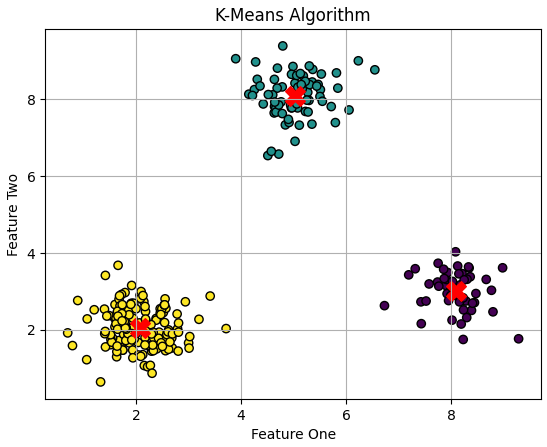
\includegraphics[width=\linewidth]{Figures/K-Means.png}
    \caption{Example of K-Means clustering on three distinct groups.}
    \label{fig:kmeans}
\end{figure}




\subsection{DC Algorithms}
%Breif review of DC functions, sufficient conditions, 
Difference of Convex Programming describes the Optimization Problem

\begin{equation}
    min \quad f(x) := g(x) - h(x), \quad \text{subject to } x \in R^d
    \label{dc function}
\end{equation}

\noindent where $g,h : R^d \;\rightarrow\; (-\infty,\infty] $ are convex. First introduced in \cite{tao_algorithms_1986} and expanded in many prolific works such has \cite{tao_convex_1997}, the resulting methods for solving these problems (know as DC algorithms(DCA)) have had use in many applications in machine learning and data science. While it it outside the scope of this work to provide a complete review of DCA, there are the following conditions. 
\begin{theorem}[Necessary condition for DCA]
 Suppose that $\bar{x}$ is a local minimizer of $f$ in \ref{dc function} then 
 \begin{equation}
 \partial h(\bar{x}) \subset \partial g(\bar{x})
\end{equation}

\label{thm:Necessary1}
\end{theorem}
\begin{theorem}[Sufficient condition for DCA]
 Suppose that there exists a neighborhood $\mathcal{N}$ of $\bar{x}$ such that 

\begin{equation}
    \varnothing \neq \partial h(x) \subset \partial g(\bar{x})
\quad\forall\,x\in \mathcal{N}.
\label{eq:suff1}
\end{equation}

\label{thm:Necessary1}
\end{theorem}

% One way of looking at this algorithm is following the traditional "guess and check" approach. After one round of centroid selection, entities are assigned to each centroid. Then the centroids are selected to minimize distance between the entities in a group and gradually that reach positions where they converge. 
% Finally, one addition from \cit{an_minimum_2009}.


% \begin{lemma}

% \cite{an_minimum_2009} Let $K$ be a nonempty bounded polyhedral convex set, $f$ be a DC function on $K$, and $p$ be a nonnegative concave function on $K$. Then there exists $t_0 \ge 0$ such that for all $t > 0$ the following problems have the same optimal value and the same solution set:
% \begin{align}
% \nonumber \quad(P) \quad \alpha = inf\{f(x):x\in K, p(x)\le 0  \} 
% \\
% \nonumber \quad \quad \quad (P_t) \quad \alpha (t) = inf\{f(x) +tp(x):x\in K, p(x)\le 0  \} 
% \end{align}
% \end{lemma}
\noindent The proofs and basic implementation of DCA for these are already covered in other works \cite{tao_convex_1997}. 
%Extensions beyond current classwork

\subsection{DCA for MSSC}
The works adapting DCA to MSSC include \cite{Ordin_heuristic_2015},\cite{artacho_boosted_nodate}, and many others outside the scope of this report. These are specifically related to rewriting equation \ref{eq:my_equatio}, as a difference of convex functions. \cite{an_minimum_2009} gives one natural adaptation. Note first that $u_{i,k} = u_{i,k}^2 \text{ as } u_{i,k} \in \{0,1\}$. 

Using the equation $f_1^2+ f_2^2 = (f_1+f_2)^2-2f_1f_2$ equation \ref{eq:my_equatio} can be rewritten as 
\[ f(U,V) = \sum_{k=1}^{n}\sum_{i=1}^{c}u_{i,k}^2 \|x_k - v_i\|^2 =\]
\[\frac{1}{2}\sum_{k=1}^{n}\sum_{i=1}^{c}(u_{i,k}^2 +\|x_k - v_i\|^2)^2-\frac{1}{2}(u_{i,k}^4+\|x_k - v_i\|^4).\]
Thus, \

\begin{equation}
    f(U,V):=G_1(U,V)-H_1(U,V)
\end{equation} 
where
\begin{equation}
G_1(U,V) = \frac{1}{2}\sum_{k=1}^{n}\sum_{i=1}^{c}(u_{i,k}^2 +\|x_k - v_i\|^2)^2
\end{equation} 
and
\begin{equation}
H_1(U,V)=\frac{1}{2}\sum_{k=1}^{n}\sum_{i=1}^{c}(u_{i,k}^4+\|x_k - v_i\|^4).
\end{equation} 

Note that each is the sum of convex functions and therefore also convex. This shows that $f(U,V)$ is a DC function. While the work \cite{an_minimum_2009} provides further information on how to adapt for implementation it comments, "this DC decomposition is not interesting because it requires an iterative algorithm for solving a convex program at each iteration."